\chapter{Resultados} % Main chapter title
\label{Chapter3 } % For referencing the chapter elsewhere, use 

\section{Evolución mensual de matrículas}

En este análisis se identificó la evolución que han tenido la cantidad de matrículas de cada mes en los últimos 3 años, las siguientes imágenes muestran la evolución por año:

\begin{figure}[th]
\centering
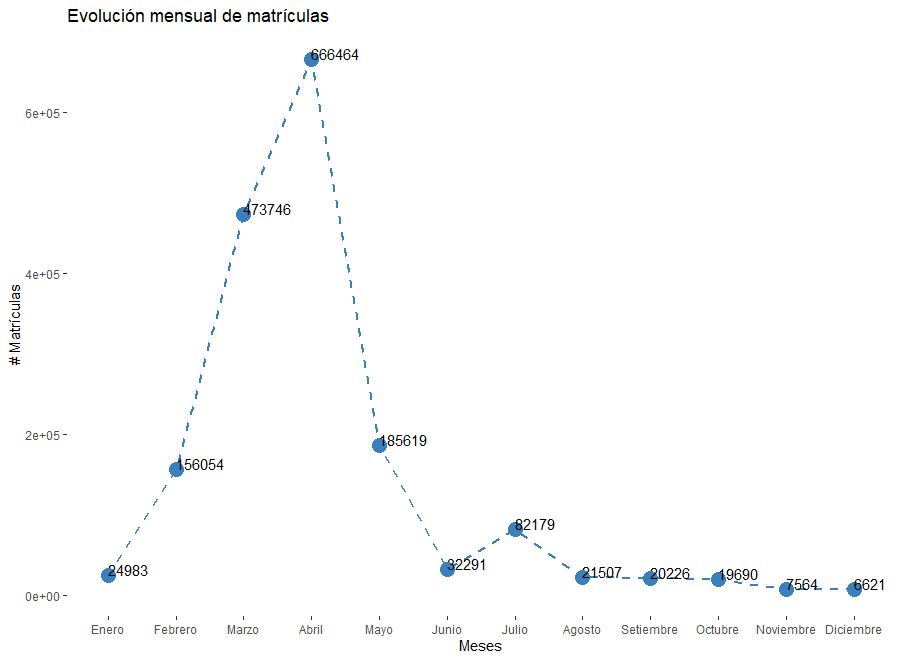
\includegraphics[width=1.2\textwidth]{Figures/matriculas2020}
\decoRule
\caption[Matrículas 2020]{Evolución de cantidades por cada mes}
\label{fig:matriculas2020}
\end{figure}

\begin{figure}[th]
\centering
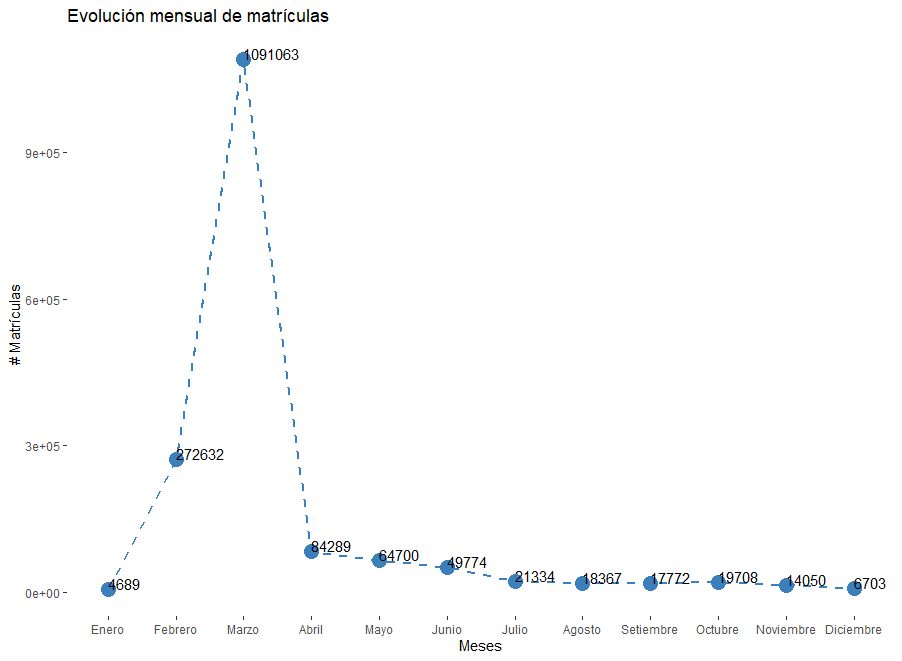
\includegraphics[width=1.2\textwidth]{Figures/matriculas2021}
\decoRule
\caption[Matrículas 2021]{Evolución de cantidades por cada mes}
\label{fig:matriculas2021}
\end{figure}

\begin{figure}[th]
\centering
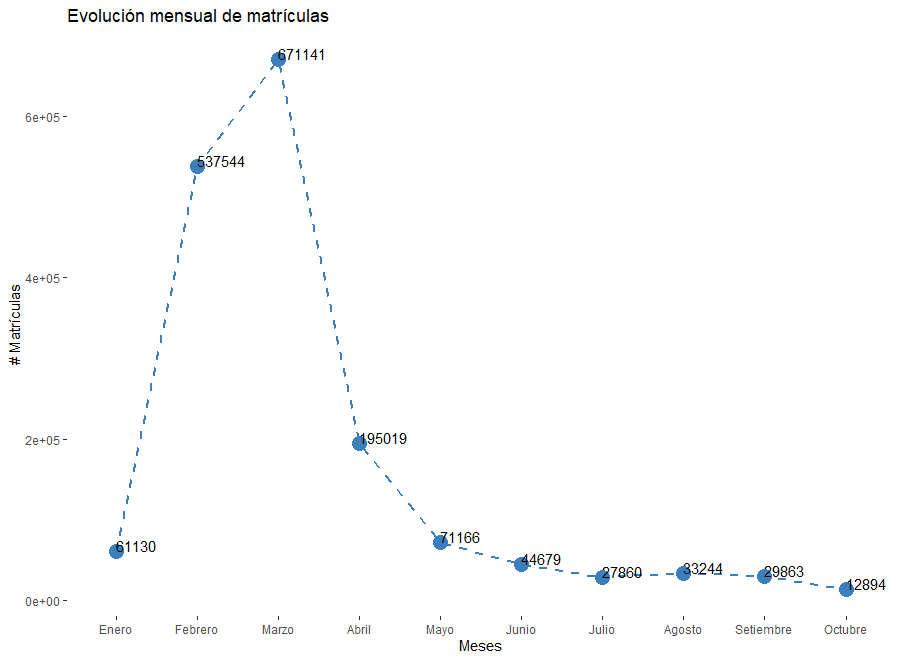
\includegraphics[width=1.2\textwidth]{Figures/matriculas2022}
\decoRule
\caption[Matrículas 2022]{Evolución de cantidades por cada mes}
\label{fig:matriculas2022}
\end{figure}

EL código de estas gráficas se encuentra en la sección \ref{evolucion_matriculas}.